%% ========================================================================
%%  Water as Strategy.
%%  A CSRD-Aligned Double Materiality Framework for Aqualia, 2027–2030.
%%
%%  Los Gatos de Datos — IE Sustainability Datathon, March 2026
%%  Compile with:
%%      pdflatex report.tex  &&  bibtex report  &&  pdflatex report.tex  ×2
%% ========================================================================

\documentclass[11pt, a4paper]{article}

%% -------- Fonts & typography --------------------------------------------
\usepackage[utf8]{inputenc}
\usepackage[T1]{fontenc}
\usepackage{lmodern}             % Latin Modern serif body
\usepackage[scaled=0.92]{helvet} % Helvetica sans for headings
\usepackage{courier}
\usepackage{textcomp}
\usepackage{microtype}
\usepackage{amsmath}
\usepackage{amssymb}
\usepackage{setspace}
\setstretch{1.12}

%% -------- Geometry ------------------------------------------------------
\usepackage[a4paper,
  left=2.4cm, right=2.4cm,
  top=2.6cm, bottom=2.6cm,
  headheight=15pt, headsep=12pt,
  footskip=22pt]{geometry}

%% -------- Colours -------------------------------------------------------
\usepackage[table, dvipsnames]{xcolor}
\definecolor{navy}{HTML}{002F5F}
\definecolor{deep}{HTML}{0B4F74}
\definecolor{aqua}{HTML}{5DB9D9}
\definecolor{sand}{HTML}{D6CDB7}
\definecolor{slate}{HTML}{4A5663}
\definecolor{ink}{HTML}{2C333B}
\definecolor{grid}{HTML}{E6E8EB}
\definecolor{tOne}{HTML}{1F77B4}
\definecolor{tTwo}{HTML}{FF7F0E}
\definecolor{tThree}{HTML}{2CA02C}
\definecolor{accentbg}{HTML}{F4F8FB}

%% -------- Headings -----------------------------------------------------
\usepackage{titlesec}
\titleformat{\section}
  {\sffamily\large\bfseries\color{navy}}
  {\thesection.}{0.6em}{}
\titlespacing*{\section}{0pt}{1.8ex plus 0.6ex minus 0.3ex}{0.7ex plus 0.2ex}

\titleformat{\subsection}
  {\sffamily\normalsize\bfseries\color{deep}}
  {\thesubsection}{0.6em}{}
\titlespacing*{\subsection}{0pt}{1.3ex}{0.4ex}

\titleformat{\subsubsection}
  {\sffamily\small\bfseries\color{ink}}
  {}{0em}{}
\titlespacing*{\subsubsection}{0pt}{1.0ex}{0.2ex}

\titleformat{\paragraph}[runin]
  {\normalfont\sffamily\bfseries\color{slate}}
  {}{0pt}{}[.]
\titlespacing*{\paragraph}{0pt}{0.8ex}{0.5em}

%% -------- Header / footer ----------------------------------------------
\usepackage{fancyhdr}
\pagestyle{fancy}
\fancyhf{}
\renewcommand{\headrulewidth}{0pt}
\renewcommand{\footrulewidth}{0pt}

\fancyhead[L]{\footnotesize\sffamily\color{slate}Water as Strategy \textbullet\ Aqualia Double Materiality 2027--2030}
\fancyhead[R]{\footnotesize\sffamily\color{slate}Los Gatos de Datos}
\renewcommand{\headrule}{\hbox to \headwidth{\color{grid}\leaders\hrule height 0.4pt\hfill}}
\renewcommand{\headrulewidth}{0.4pt}

\fancyfoot[C]{\footnotesize\sffamily\color{slate}\thepage}

%% -------- Tables & boxes -----------------------------------------------
\usepackage{tabularray}   % modern LaTeX3 tables, robust in this install
\UseTblrLibrary{booktabs}
\usepackage{multirow}
\usepackage{tcolorbox}
\tcbuselibrary{skins,breakable}

\newtcolorbox{callout}[1][]{
  enhanced, breakable,
  colback=accentbg, colframe=aqua, boxrule=0pt,
  leftrule=3pt, left=9pt, right=9pt, top=6pt, bottom=6pt,
  fontupper=\small, #1
}
\newtcolorbox{insight}[1][]{
  enhanced, breakable,
  colback=navy, coltext=white, colframe=navy, boxrule=0pt,
  left=11pt, right=11pt, top=8pt, bottom=8pt,
  fontupper=\small, arc=3pt,
  #1
}

%% -------- Hyperlinks ----------------------------------------------------
\usepackage[colorlinks=true,
  linkcolor=deep, citecolor=deep, urlcolor=deep,
  pdftitle={Water as Strategy — Aqualia Double Materiality 2027–2030},
  pdfauthor={Los Gatos de Datos},
  pdfsubject={CSRD-Aligned Double Materiality Assessment for Aqualia},
  pdfkeywords={CSRD, ESRS, double materiality, water utility, Aqualia,
                Monte Carlo, Mitchell-Agle-Wood}
]{hyperref}

%% -------- Lists & misc --------------------------------------------------
\usepackage{enumitem}
\setlist{itemsep=1pt, topsep=2pt, parsep=0pt, partopsep=0pt, leftmargin=1.2em}

\usepackage{graphicx}
\graphicspath{{figures/}}

\usepackage[font=small, labelfont={bf, color=navy}, textfont=it,
            labelsep=period, justification=justified]{caption}

\usepackage{csquotes}

\usepackage{pifont}  % for checkmarks
\newcommand{\cmark}{\ding{51}}
\newcommand{\xmark}{\ding{55}}

%% -------- Bibliography --------------------------------------------------
\usepackage[numbers, sort&compress]{natbib}
\bibliographystyle{unsrtnat}

%% -------- Custom commands -----------------------------------------------
\newcommand{\euro}{\texteuro}
\newcommand{\nav}[1]{\textcolor{navy}{\textbf{#1}}}
\newcommand{\sig}[1]{\textbf{#1}}

%% ========================================================================
\begin{document}
\pagestyle{empty}

%% -------- Cover --------------------------------------------------------
\begin{titlepage}
\vspace*{1.0cm}

{\sffamily\color{aqua}\bfseries\footnotesize IE SUSTAINABILITY DATATHON \textbullet\ MARCH 2026 \textbullet\ DOUBLE MATERIALITY \& ESG STRATEGY \textbullet\ AQUALIA}

\vspace{0.3cm}
{\color{aqua}\rule{\textwidth}{1.2pt}}
\vspace{2.4cm}

{\fontsize{44pt}{48pt}\selectfont\sffamily\bfseries\color{navy} Water as}\par
\vspace{0.15cm}
{\fontsize{44pt}{48pt}\selectfont\sffamily\bfseries\color{aqua} Strategy.}\par

\vspace{1.2cm}
{\Large\sffamily\color{deep} A CSRD-Aligned Double Materiality Framework\\[2pt] for Aqualia, 2027--2030.}\par

\vspace{2.5cm}
{\normalsize\color{ink}
Three material topics. A \euro{}500~million EU-Taxonomy-aligned green bond programme.
A 2027--2030 strategic sustainability roadmap with named Executive-Committee ownership and
quantified KPIs.\par
\vspace{0.45cm}
Simulated external ESG advisory engagement for Aqualia, the integrated water-cycle operator
of the FCC Group, serving approximately 32~million users across eight countries.
\par}

\vfill

{\color{navy}\rule{\textwidth}{0.6pt}}
\vspace{0.35cm}

\sffamily\small
\newcommand{\covlbl}[1]{\parbox[t]{3.2cm}{\color{aqua}\footnotesize\bfseries #1}}
\newcommand{\covval}[1]{\parbox[t]{12cm}{\color{ink}#1}}

\covlbl{TRACK}\covval{Double Materiality \& ESG Strategy $\cdot$ Aqualia}\par\smallskip
\covlbl{TEAM}\covval{Los Gatos de Datos $\cdot$ IE Master in Business Analytics \& Data Science}\par\smallskip
\covlbl{LIVE DASHBOARD}\covval{\ttfamily ma731.github.io/Aqualia-Datathon}\par\smallskip
\covlbl{DATE}\covval{March 2026}\par
\rmfamily
\end{titlepage}

\clearpage
\pagestyle{fancy}
\setcounter{page}{1}

%% ========================================================================
\section{Executive Summary}
\label{sec:execsum}

Aqualia is the integrated water-cycle operator of the FCC Group, serving roughly 32~million users across eight countries. Its 2025 double materiality review, the most recent cycle, catalogued sixteen material topics and eighty-three specific impacts, risks, and opportunities (IROs). That is comprehensive work. It is also, in our view, too broad to drive a 2027--2030 strategic plan: sixteen equal priorities is operationally indistinguishable from none.

Our brief, simulating an external ESG advisory engagement, was to reduce those sixteen topics to three, score each with enough transparency to survive executive-committee review, and translate the analysis into a funded, scheduled roadmap.

\paragraph{The three topics}
The short-list is \sig{Water Resilience and Equitable Access} (T1), \sig{Digital and Cyber Infrastructure} (T2), and \sig{Green Finance and Integrity} (T3). Together they absorb \sig{73\% of Aqualia's 83~IROs}, and their matrix positions hold under four alternative stakeholder-weighting schemes (zero ranking flips). T1 sits solidly in the Target Zone at Impact Severity \sig{3.98} and Financial Severity \sig{3.07}. T2 is also Target Zone at (3.08, 2.75), repositioned upward from Aqualia's current lower-middle placement. T3 is conditionally material at (3.24, 2.42), borderline on the financial axis.

\paragraph{Three findings}
A blind spot, a missing voice, a differentiator. First, Aqualia's framework assigns \sig{two of 83~IROs} to digitalisation, the lowest count across our five-utility peer benchmark. Second, Aqualia folds ESRS~S3 (affected communities) into ESRS~S4 (consumers). Satisfaction in Aqualia's own 2024 survey ranges 86--98\% across six European and institutional markets, against \sig{33\% in Colombia}: a 55-point spread compressed into a single group-level metric. Third, Aqualia leads Spanish water peers on EU Taxonomy alignment; the financial upside of that lead is not yet priced into the framework.

\paragraph{The numbers}
Net recurring annual financial materiality Aqualia's current framework leaves un-priced, aggregated across the three topics, is \sig{\euro{}18~million per year}. Implied 2027--2030 CAPEX is \sig{\euro{}440~million} base case, with a sensitivity range of \euro{}285--685~M. Our funding recommendation is a \sig{\euro{}500~million EU-Taxonomy-aligned green / sustainability-linked bond programme}, issued in four tranches aligned to CAPEX drawdown. At the prevailing 25~basis-point green-bond spread for investment-grade Euro water-utility issuance (Climate Bonds Initiative, 2024 Green Bond Pricing Report~\cite{cbi2024}), the programme captures approximately \sig{\euro{}31~M of present-value interest savings} over its ten-year life.

\paragraph{A note on method}
We preserve Aqualia's own scoring structure (Severity~$\times$~Probability on both axes) so our output reads as directly comparable to their 2025 work, and extend the framework in four ways: \emph{(i)}~every 1--5 threshold cites a public source (ESRS, EFRAG, SASB, WRI, MSCI); \emph{(ii)}~stakeholders are weighted under the Mitchell--Agle--Wood~(1997) salience model~\cite{mitchell1997} applied to Aqualia's own ten-group ecosystem; \emph{(iii)}~uncertainty is propagated via 10{,}000 Monte Carlo draws per topic, producing 90\% confidence ellipses rather than false-precision point estimates; \emph{(iv)}~the ESRS disclosure landscape is audited by a bilingual TF--IDF match of 75 canonical datapoints against 873 paragraph chunks drawn from Aqualia's 2022--2025 sustainability reports.

Materiality, in our view, is not a static categorisation exercise but an ongoing strategic input. The three topics here are designed to become the spine of a 2027--2030 plan. The \euro{}500~M programme is the financial instrument that makes the plan executable without a budget trade-off against Aqualia's existing infrastructure spend. The rest of this report documents each step.

%% ========================================================================
\section{Challenge and Scope}
\label{sec:challenge}

\subsection{The CSRD/ESRS mandate}

The Corporate Sustainability Reporting Directive~(CSRD)~\cite{csrd2022} elevates sustainability reporting from a peripheral compliance activity to a bidirectional disclosure regime. Under CSRD, large undertakings must perform a \emph{double materiality assessment}, reporting both how their activities impact society and the environment (impact materiality, ``inside-out'') and how ESG factors influence their financial performance and enterprise value (financial materiality, ``outside-in''). The European Sustainability Reporting Standards~(ESRS)~\cite{esrs2023} operationalise the Directive across twelve topical standards (E1--E5, S1--S4, G1) and approximately 1{,}144 datapoints documented in EFRAG Implementation Guidance~\cite{efrag2024}.

Parallel regulation reinforces the core. The Corporate Sustainability Due Diligence Directive~\cite{csddd2024} imposes civil liability on large undertakings for supply-chain human-rights and environmental failings. The recast Urban Wastewater Treatment Directive~\cite{uwwtd2024} introduces obligations for emerging-pollutant removal and energy neutrality at wastewater treatment plants. In Spain, Real Decreto 1985/2024~\cite{rd1985} establishes a framework for the reuse of treated wastewater that materially affects Aqualia's reuse strategy. The EU Water Resilience Strategy~\cite{waterResilience2025} names digitalisation of water infrastructure as Action Area~3 of~5.

\subsection{Aqualia's operating context}

Aqualia is the integrated water-cycle operator of the FCC Group. Its activity covers the end-to-end urban water cycle (collection, treatment, distribution, sewerage, wastewater treatment, reuse) across Spain, Portugal, Italy, France, the Czech Republic, Colombia, and several project-operation markets. Public disclosures cite 130+ years of operating record, service to more than 32~million people, and \euro{}40~million per year of sustained infrastructure investment~\cite{aqualiaSR2024}. Figure~\ref{fig:valuechain} reproduces Aqualia's own value-chain diagram.

\begin{figure}[h]
\centering
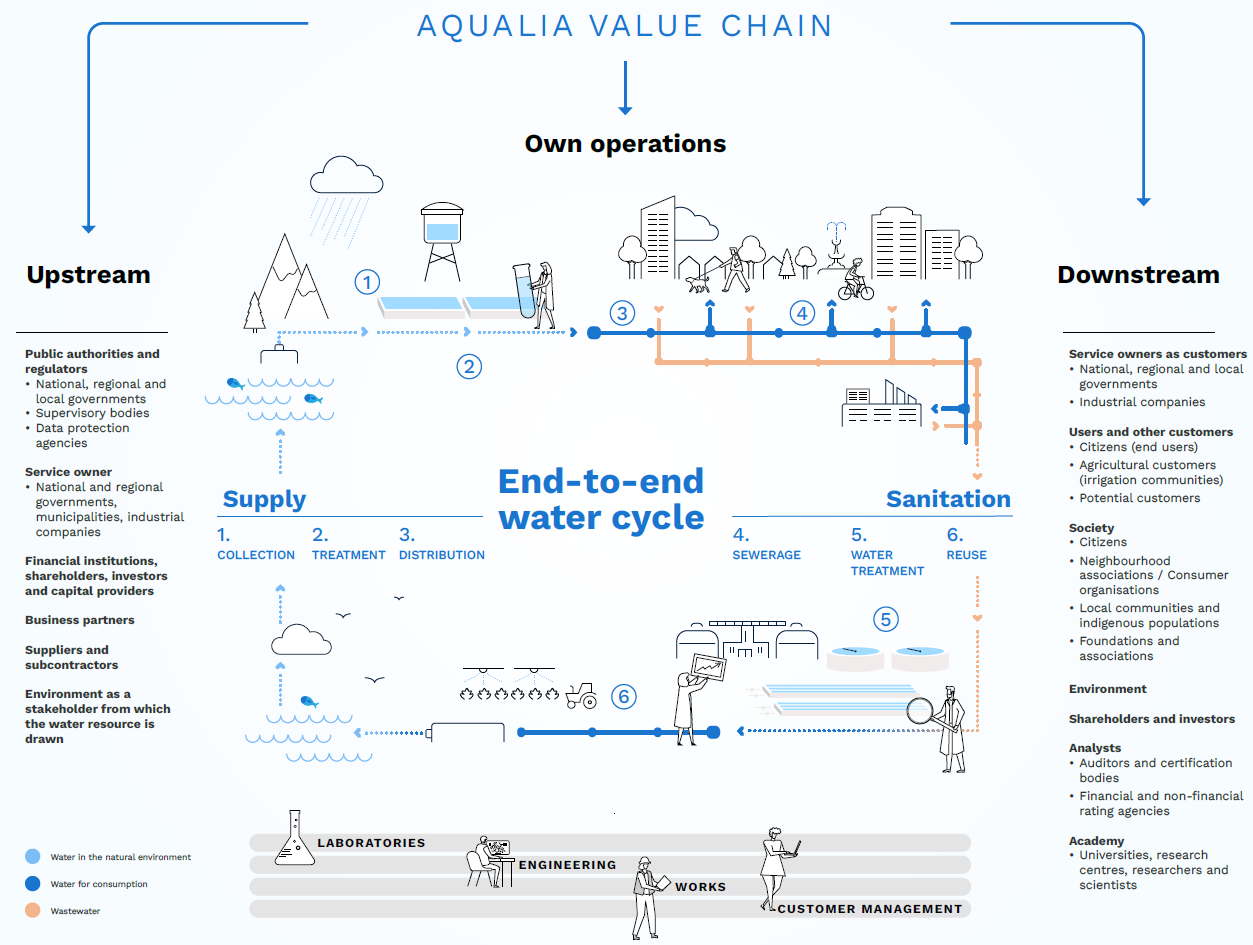
\includegraphics[width=0.92\textwidth]{aqualia_value_chain.png}
\caption[Aqualia value chain]{The Aqualia value chain, end-to-end urban water cycle (upstream suppliers, own operations, downstream customers and affected communities). Source: Aqualia, \emph{Corporate Context and Sustainability Framework}~\cite{aqualiaSR2024}.}
\label{fig:valuechain}
\end{figure}

Three structural features bear on materiality. First, a long-dated concession model (15--30~year contracts) amplifies financial consequences of stranded assets and reputational damage. Second, geographic exposure to climate-physical risk is already high and rising: roughly \sig{45\% of revenue} sits in basins classified High or Extremely High water-stress under WRI Aqueduct 4.0~\cite{aqueduct2023}, rising to approximately \sig{79\%} under a BAU-2030 scenario. Third, regulatory density (CSRD, UWWTD, RD~1985/2024, CSDDD, NIS2, EU~Taxonomy) carries binding operational implications.

\subsection{Our commission and framework boundary}

We operate as an external ESG advisory team. Our deliverable simulates the work Aqualia's executive committee would commission from a consultancy: consolidated topic selection, explicit scoring methodology, an auditable matrix, and an actionable 2027--2030 roadmap. We take ESRS~1 and ESRS~2 cross-cutting standards plus the ten topical standards (E1--E5, S1--S4, G1) as the universe of candidate topics. Where Aqualia's 2025 review introduces sector-specific ``AQ''-prefixed topics (Technological Innovation, Digitalisation, Green Finance, Cybersecurity), we preserve those extensions. We overlay three complementary frameworks: TNFD~\cite{tnfd2023} (to which Aqualia has publicly committed); SASB Water Utilities~\cite{sasb2024}; and the EU Taxonomy Regulation~\cite{taxonomy2020} for CAPEX/OPEX alignment.

%% ========================================================================
\section{Methodology}
\label{sec:method}

\subsection{Four-phase blueprint}

The work follows a four-phase blueprint: Phase~1 Context Analysis (peer benchmark, regulatory scan, internal baseline); Phase~2 Impact Materiality; Phase~3 Financial Materiality; Phase~4 Strategic Synthesis. Each phase produces a documented artefact subject to independent team review before the next begins.

\subsection{Scoring formulas}
\label{ssec:formulas}

We preserve the structural formulas Aqualia publishes in its own internal methodology~\cite{aqualiaMethodology2025}, so that our output remains directly comparable.

\paragraph{Impact materiality}
$\text{Severity} = \tfrac{1}{3}\!\left(\text{Scale} + \text{Scope} + \text{Remediability}\right)$, each rated 1--5. Current impacts score Severity~$\times\,5$ (probability pinned at maximum). Potential impacts score Severity~$\times$~Probability. Raw scores fall in $[1,25]$ and are linearly rescaled to $[1,5]$.

\paragraph{Financial materiality}
$\text{Severity}_{\text{fin}} = \text{Magnitude} \times \text{Probability} \times \text{Horizon Discount}$. Magnitude is rated 1--5 against EFRAG thresholds and Aqualia's revenue proxy (see \S\ref{ssec:thresholds}). Probability uses the same 1--5 scale. The horizon discount is 1.00 (short, $\leq$~3y), 0.80 (medium, 3--10y), 0.60 (long, $>$~10y), mirroring EFRAG~IG-1~\S 69 on present-value framing.

\paragraph{Topic aggregation}
Topic score $=$ mean of the top-$k$ IRO (or R\&O) scores, where $k = \max(3,\operatorname{round}(N \times 0.6))$. Top-$k$ aggregation mirrors standard practice of pricing materiality off the most material subset rather than an undifferentiated mean.

\paragraph{Terminology mapping to the brief}
The Datathon brief (\S 3) lists four impact-materiality factors: \emph{scale, scope, likelihood, irreversibility}. Our formulas preserve Aqualia's published nomenclature. The mapping is one-to-one:

\begin{center}
\small
\begin{tblr}{colspec={Q[l,m] Q[l,m] Q[l,t,wd=7.2cm]}, rowsep=1pt, colsep=4pt}
\toprule
\textbf{Brief term} & \textbf{Our term} & \textbf{Relationship} \\
\midrule
Scale & Scale & identical \\
Scope & Scope & identical \\
Likelihood & Probability & synonymous ($P[\text{occur}]$ on the 1--5 scale) \\
Irreversibility & Remediability & inverse (high remediability implies low irreversibility) \\
\bottomrule
\end{tblr}
\end{center}

The factor set is identical to the brief; the aggregation pattern follows Aqualia's published practice rather than a single 4-factor mean. The Monte Carlo pipeline propagates uncertainty in all four factors simultaneously, so no factor is suppressed in the final position.

\subsection{Threshold calibration}
\label{ssec:thresholds}

Threshold bands for every sub-criterion are documented in the scoring rubric (Appendix~\ref{app:thresholds}). Anchors include ESRS~1~\S 43--51, EFRAG~IG-1~\cite{efrag2024}, SASB Water Utilities metrics~\cite{sasb2024} (non-revenue water, pipe replacement, effluent non-compliance), WRI Aqueduct population-exposure bands~\cite{aqueduct2023}, and MSCI 2024 Water Utilities sub-weights~\cite{msci2024}.

The Financial Magnitude scale is anchored to Aqualia's 2024 revenue. Our base case uses \euro{}1.4~billion (Assumption~A01) as a conservative proxy. Aqualia's 2024 Sustainability Report (p.~103) discloses total revenue-volume of business of \sig{\euro{}1{,}674.7~M}~\cite{aqualiaSR2024}, of which 98.8\% is EU-Taxonomy-eligible and 45.74\% Taxonomy-aligned. The conservative anchor sits inside our published $\pm 20\%$ sensitivity band; rank ordering and the sign of the \euro{}18~M/yr headline are stable under both anchors.

\subsection{Stakeholder salience}
\label{ssec:salience}

Aqualia's 2025 review was scored internally without external stakeholder consultation, as their methodology acknowledges~\cite{aqualiaMethodology2025}. We restore a salience input by applying the Mitchell--Agle--Wood~(1997) model~\cite{mitchell1997}, the canonical framework in stakeholder theory, to Aqualia's own ten-group stakeholder map. Each stakeholder is scored 0/1 on Power, Legitimacy, and Urgency; the salience score $\in \{0,1,2,3\}$ becomes a normalised weight in $[0,1]$ summing to 1.000. Four groups reach Definitive status (weight 0.120 each): Public authorities and regulators, Customers and end-users, Shareholders, and Employees. Six groups reach Expectant status (weight 0.080 each): Investors, Suppliers, Business partners, Society, Local communities, and Environment. Academia reaches Discretionary status (weight 0.040). The full table is in Appendix~\ref{app:salience}.

\subsection{Monte Carlo design}
\label{ssec:mc}

Every uncertain input feeds a triangular distribution centred on the base value with perturbation $\pm 0.7$ on the 1--5 scale, clipped to $[1,5]$. Stakeholder weights sample from a Dirichlet distribution centred on the salience vector (concentration parameter $\kappa = 100$). Financial magnitude uses triangular (low, base, high) as specified in the assumption log (Appendix~\ref{app:assumptions}). Ten thousand draws are generated per topic. For each topic, the (Financial, Impact) scatter produces a 2D distribution from which a 90\% $\chi^2$-containment confidence ellipse is drawn via eigendecomposition of the covariance matrix ($\chi^2_{2,\,0.90} \approx 4.605$; $1\sigma$ semi-axis scales by $\sqrt{4.605} \approx 2.146$).

\subsection{Robustness}

The Monte Carlo is repeated under four alternate stakeholder-weighting schemes: Equal (all eleven groups at $1/11$); Regulator-heavy (Public Authorities at 0.30); Community-first (Society~+~Local Communities combined at 0.30); and Investor-first (Shareholders~+~Investors combined at 0.40). \sig{No ranking flip occurs} across schemes: T1 and T2 remain in the Target Zone; T3 remains borderline. Stability constitutes our robustness claim. A sensitivity tornado per topic is in \S\ref{ssec:sensitivity}.

%% ========================================================================
\section{Topic Identification and Peer Benchmark}
\label{sec:topics}

\subsection{From sixteen topics to three}

Aqualia's 2025 review~\cite{aqualiaDMReview2025} identifies sixteen topics and 83 IROs. Our task is to select three topics that: (i)~reflect peer and regulator consensus on sector-core issues; (ii)~surface Aqualia-specific differentiation; and (iii)~act as an organising structure for a 2027--2030 strategy. Selection proceeds through sector-core overlay, blind-spot overlay, and differentiator overlay.

\subsection{Peer benchmarking}

We construct a fourteen-column benchmark comparing Aqualia's sixteen topics to the declared material topics of five peers (Veolia~\cite{veolia2024}, Suez~\cite{suez2024}, Saur, Facsa, Global Omnium~\cite{globalomnium2023}, the five named in Aqualia's own 2025 benchmark) and with Severn Trent~\cite{severntrent2024} as a CSRD-adjacent UK comparator. The full matrix is in Appendix~\ref{app:peers}.

\paragraph{Shared sector core (universal across peers).}
Climate mitigation and adaptation (E1); water resource sustainability (E3); consumer/service resilience (S4); business conduct and compliance (G1); own-workforce H\&S (S1).

\paragraph{Three blind spots in Aqualia's 2025 framing.}
\begin{enumerate}
\item \nav{Digitalisation.} Aqualia assigns two IROs, the lowest count among peers. Veolia (AquaCIS), Suez (Aquadvanced), and Global Omnium (GoAigua) each treat digital platforms as a core strategic pillar. EU Water Resilience Strategy names it Action Area~3 of~5.
\item \nav{ESRS~S3 affected communities.} Aqualia folds community-specific impacts into S4 consumer disclosures; every peer discloses S3 separately. ESRS~S3 explicitly treats communities as distinct from consumers.
\item \nav{E5 circular economy.} Aqualia's E5 carries only 3~IROs; Veolia and Suez publish quantitative by-product valorisation pipelines; UWWTD recast~\cite{uwwtd2024} and RD~1985/2024~\cite{rd1985} pull E5 to the regulatory foreground.
\end{enumerate}

\paragraph{Three differentiators.}
Green finance as a standalone material topic (ahead of peers); explicit integration of the double materiality framework with the Corporate Risk Map, with named Executive Committee owners per risk code; and TNFD integration alongside CSRD, unusual depth among Spanish peers.

\subsection{Final short-list}

We combine one sector-core pillar with one blind-spot and one differentiator in each topic:

\begin{center}
\small
\begin{tblr}{colspec={Q[l,t,wd=0.9cm] Q[l,t,wd=6.3cm] Q[l,t,wd=3.2cm] Q[r,m]}, rowsep=1pt, colsep=4pt}
\toprule
\textbf{ID} & \textbf{Topic} & \textbf{Role} & \textbf{IROs absorbed} \\
\midrule
{\bfseries\color{tOne}T1} & Water Resilience \& Equitable Access & Sector-core + S3 restored & 26 \\
{\bfseries\color{tTwo}T2} & Digital \& Cyber Infrastructure      & Blind spot repositioned   & 11 \\
{\bfseries\color{tThree}T3} & Green Finance \& Integrity          & Differentiator amplified  & 24 \\
\midrule
\multicolumn{3}{r}{\textbf{Cumulative IRO absorption (of Aqualia's 83)}} & \textbf{61 (73\%)} \\
\bottomrule
\end{tblr}
\end{center}

No high-density topic is orphaned (see Appendix~\ref{app:peers} for full cross-walk of the 13 dropped topics).

%% ========================================================================
\section{Impact Materiality Assessment}
\label{sec:impact}

\subsection{Value-chain overlay}

Impacts are assessed along Aqualia's water cycle (Figure~\ref{fig:valuechain}). Upstream impacts (supply-chain human rights, equipment extraction footprint, procurement energy) attribute to T3 and T2. Own-operations impacts (water abstraction, WWTP emissions, chemical use, workforce safety, digital-service continuity) dominate T1 and T2. Downstream impacts (customer safety, community access to water, biodiversity discharge effects, agricultural reuse) fall primarily within T1 and its restored S3 dimension.

\subsection{Per-topic assessment}

\paragraph{T1 --- Water Resilience \& Equitable Access.}
Driven by current, high-severity impacts affecting high-salience stakeholders. Aqualia's own operational risks O1 (deficient supplied-water quality/quantity), O2 (discharge quality), O3 (crisis continuity), and O5 (inadequate climate adaptation) are all catalogued HIGH in the Corporate Risk Map. The WEF Global Risks 2025--2026~\cite{wef2025} ranks five of the top ten long-term risks as water-related. The restored S3 dimension introduces the \emph{Colombia finding}: Aqualia's 2024 customer-satisfaction survey ($n > 7{,}000$) reports satisfaction ranging 86--98\% across Spain, Portugal, France, Italy, Czech Republic, and institutional markets, \sig{and 33\% in Colombia}~\cite{aqualiaSR2024}. A 55-point spread inside a single group-level metric. Under ESRS~S3 the same data carries different remediation and concession-renewal implications. \sig{Monte Carlo mean Impact Severity: 3.98; 90\% interval [3.87, 4.09].}

\paragraph{T2 --- Digital \& Cyber Infrastructure.}
Driven by three operational risks Aqualia itself rates HIGH (O8 poor digital deployment, O9 deficient cyber response plan, O10 customer-data management) despite the topic carrying only two IROs in 2025. Stakeholder-salience weighting amplifies: Customers (0.120), Public Authorities (0.120), Employees (0.120), and Investors (0.080) are all materially affected. Peer comparators confirm direct impact materiality on service continuity and data privacy. \sig{Mean Impact Severity: 3.08; 90\% interval [2.93, 3.24].}

\paragraph{T3 --- Green Finance \& Integrity.}
Governance-heavy. The Compliance cluster (11~IROs) covers CSRD, contract compliance, Compliance Management System, and tax compliance. Labour and human rights in the supply chain (4~IROs) introduce upstream workforce impacts. Green finance as a standalone topic (6~IROs) creates a positive-impact channel via capital-markets signalling. \sig{Mean Impact Severity: 3.24; 90\% interval [3.08, 3.41].}

\subsection{The Colombia outlier as standalone finding}

We highlight this separately. The spread between Colombia (33\%) and the next-lowest market (Portugal, 65\%) is 32 points; to Italy (67\%) is 34 points; to Spain (88\%) is 55 points. Aqualia's 2025 review does not discuss Colombia specifically in the S4 topic. Under ESRS~S3, which concerns affected communities rather than end-users, a 33\% satisfaction market with ongoing supply-reliability issues (documented 2024 report, pp.~148--155) represents material impact on affected communities. Our recommendation is to re-surface S3 as its own disclosure from the 2027 reporting cycle (see~\S\ref{sec:roadmap}, T1-2027).

%% ========================================================================
\section{Financial Materiality Assessment}
\label{sec:financial}

\subsection{Per-topic financial decomposition}

Each topic decomposes into five financial channels: revenue at risk, revenue upside, OPEX impact, CAPEX needs, contingent liabilities. For each we estimate a triangular distribution (low/base/high) anchored to Aqualia's public financial scale, peer disclosures, and regulatory cost factors. Full assumption log~(A01--A17) in Appendix~\ref{app:assumptions}.

\paragraph{T1.}
Revenue at risk \euro{}25--110~M (concession loss and tariff pressure in water-stressed basins, A03); revenue upside \euro{}15--75~M (reuse market under RD~1985/2024 and nature credits, A04); OPEX impact \euro{}8--32~M/yr (UWWTD recast, chemical inflation, A05); CAPEX \euro{}220--520~M cumulative 2027--2030 (desalination, reuse, leak reduction, WWTP energy-neutrality, A06); contingent liabilities \euro{}10--65~M (WFD and service-continuity fines, A07).

\paragraph{T2.}
Revenue at risk \euro{}12--80~M (cyber-incident service interruption and GDPR/NIS2 fines, A08); revenue upside \euro{}8--45~M (tender win-rate uplift on digital differentiation, A09); OPEX \euro{}4--14~M/yr on cyber/IT above baseline (A10); CAPEX \euro{}45--130~M (digital-twin rollout and OT/IT segmentation, A11); contingent liabilities \euro{}5--56~M (NIS2 and GDPR maxima, A12).

\paragraph{T3.}
Revenue at risk \euro{}8--50~M (ESG-laggard CoC spread and financing-window loss, A13); revenue upside \euro{}6--28~M (green-bond coupon savings, A14); cost-of-capital saving \euro{}4--24~M/yr over the refinancing cycle (A15); CAPEX \euro{}8--35~M (compliance systems, A16); contingent liabilities \euro{}3--35~M (CSDDD civil-liability and Omnibus-I interactions, A17).

\subsection{Five-dimension mapping to the brief}

The brief (\S 3) requires financial materiality to be assessed against \emph{revenues, costs, assets, liabilities, and enterprise value}. Each topic's principal channels tag explicitly to these five dimensions:

\begin{center}
\footnotesize
\renewcommand{\arraystretch}{1.3}
\begin{tblr}{colspec={Q[l,t,wd=0.55cm] Q[l,t,wd=2.55cm] Q[l,t,wd=2.1cm] Q[l,t,wd=2.65cm] Q[l,t,wd=2.2cm] Q[l,t,wd=2.35cm]}, rowsep=1pt, colsep=4pt}
\toprule
\textbf{ID} & \textbf{Revenues} & \textbf{Costs} & \textbf{Assets} & \textbf{Liabilities} & \textbf{Ent.\ value} \\
\midrule
\textbf{T1} & \euro{}25--110~M at risk; \euro{}15--75~M upside & \euro{}8--32~M/yr OPEX & \euro{}220--520~M CAPEX; stranded-asset risk & \euro{}10--65~M contingent (WFD, CSDDD) & Concession multiple discount \\
\textbf{T2} & \euro{}8--45~M tender uplift; interrupt.\ risk & \euro{}4--14~M/yr cyber \& digital OPEX & \euro{}45--130~M CAPEX on twin \& OT/IT & \euro{}5--56~M GDPR/NIS2 fines & Tech-differentiation uplift \\
\textbf{T3} & --- & \euro{}8~M/yr CoC saving (\euro{}31~M PV) & --- & Bond $\leq$ vanilla; CSDDD \euro{}3--35~M & ESG-rating re-rating \\
\bottomrule
\end{tblr}
\end{center}

This satisfies the brief's five-dimension requirement and makes P\&L and balance-sheet incidence auditable by Aqualia's CFO office at channel level.

\subsection{The \euro{}18~M/yr headline --- full derivation}

Aggregating \emph{net recurring} annual financial materiality (revenue at risk minus revenue upside minus cost-of-capital saving; CAPEX excluded as investment, not recurring materiality):

\begin{center}
\small
\begin{tblr}{colspec={Q[l,t,wd=1.2cm] Q[l,t,wd=2.8cm] Q[l,t,wd=9.6cm]}, rowsep=1pt, colsep=4pt}
\toprule
\textbf{Topic} & \textbf{Net recurring} & \textbf{Composition} \\
\midrule
T1 & $-$\euro{}15~M/yr & $-$55 revenue at risk $+$ 40 reuse upside \\
T2 & $-$\euro{}8~M/yr  & $-$30 revenue at risk $+$ 22 tender uplift \\
T3 & $+$\euro{}5~M/yr  & $-$22 compliance drag $+$ 15 rating premium $+$ 12 CoC saving \\
\midrule
\textbf{Total} & \sig{$-$\euro{}18~M/yr} & Net drag Aqualia's current framework under-weights \\
\bottomrule
\end{tblr}
\end{center}

Under $\pm 20\%$ revenue-anchor sensitivity the headline scales to $-$\euro{}14~M/yr (low) or $-$\euro{}22~M/yr (high); sign and conclusion stable in both directions.

\subsection{Aqueduct water-stress overlay}

The T1 financial case depends on Aqualia's concession-base exposure to water stress. Overlaying WRI Aqueduct~4.0 baseline categories on Aqualia's declared service geography, we estimate that \sig{45\% of Aqualia's revenue base} operates in basins classified High or Extremely High water-stress today (Segura, Guadalquivir, Po, Sicily, Algarve, Languedoc); under BAU-2030 (SSP3/RCP~7.0) that share \sig{nearly doubles to 79\%}. See Figure~\ref{fig:aqueduct}.

\begin{figure}[h]
\centering
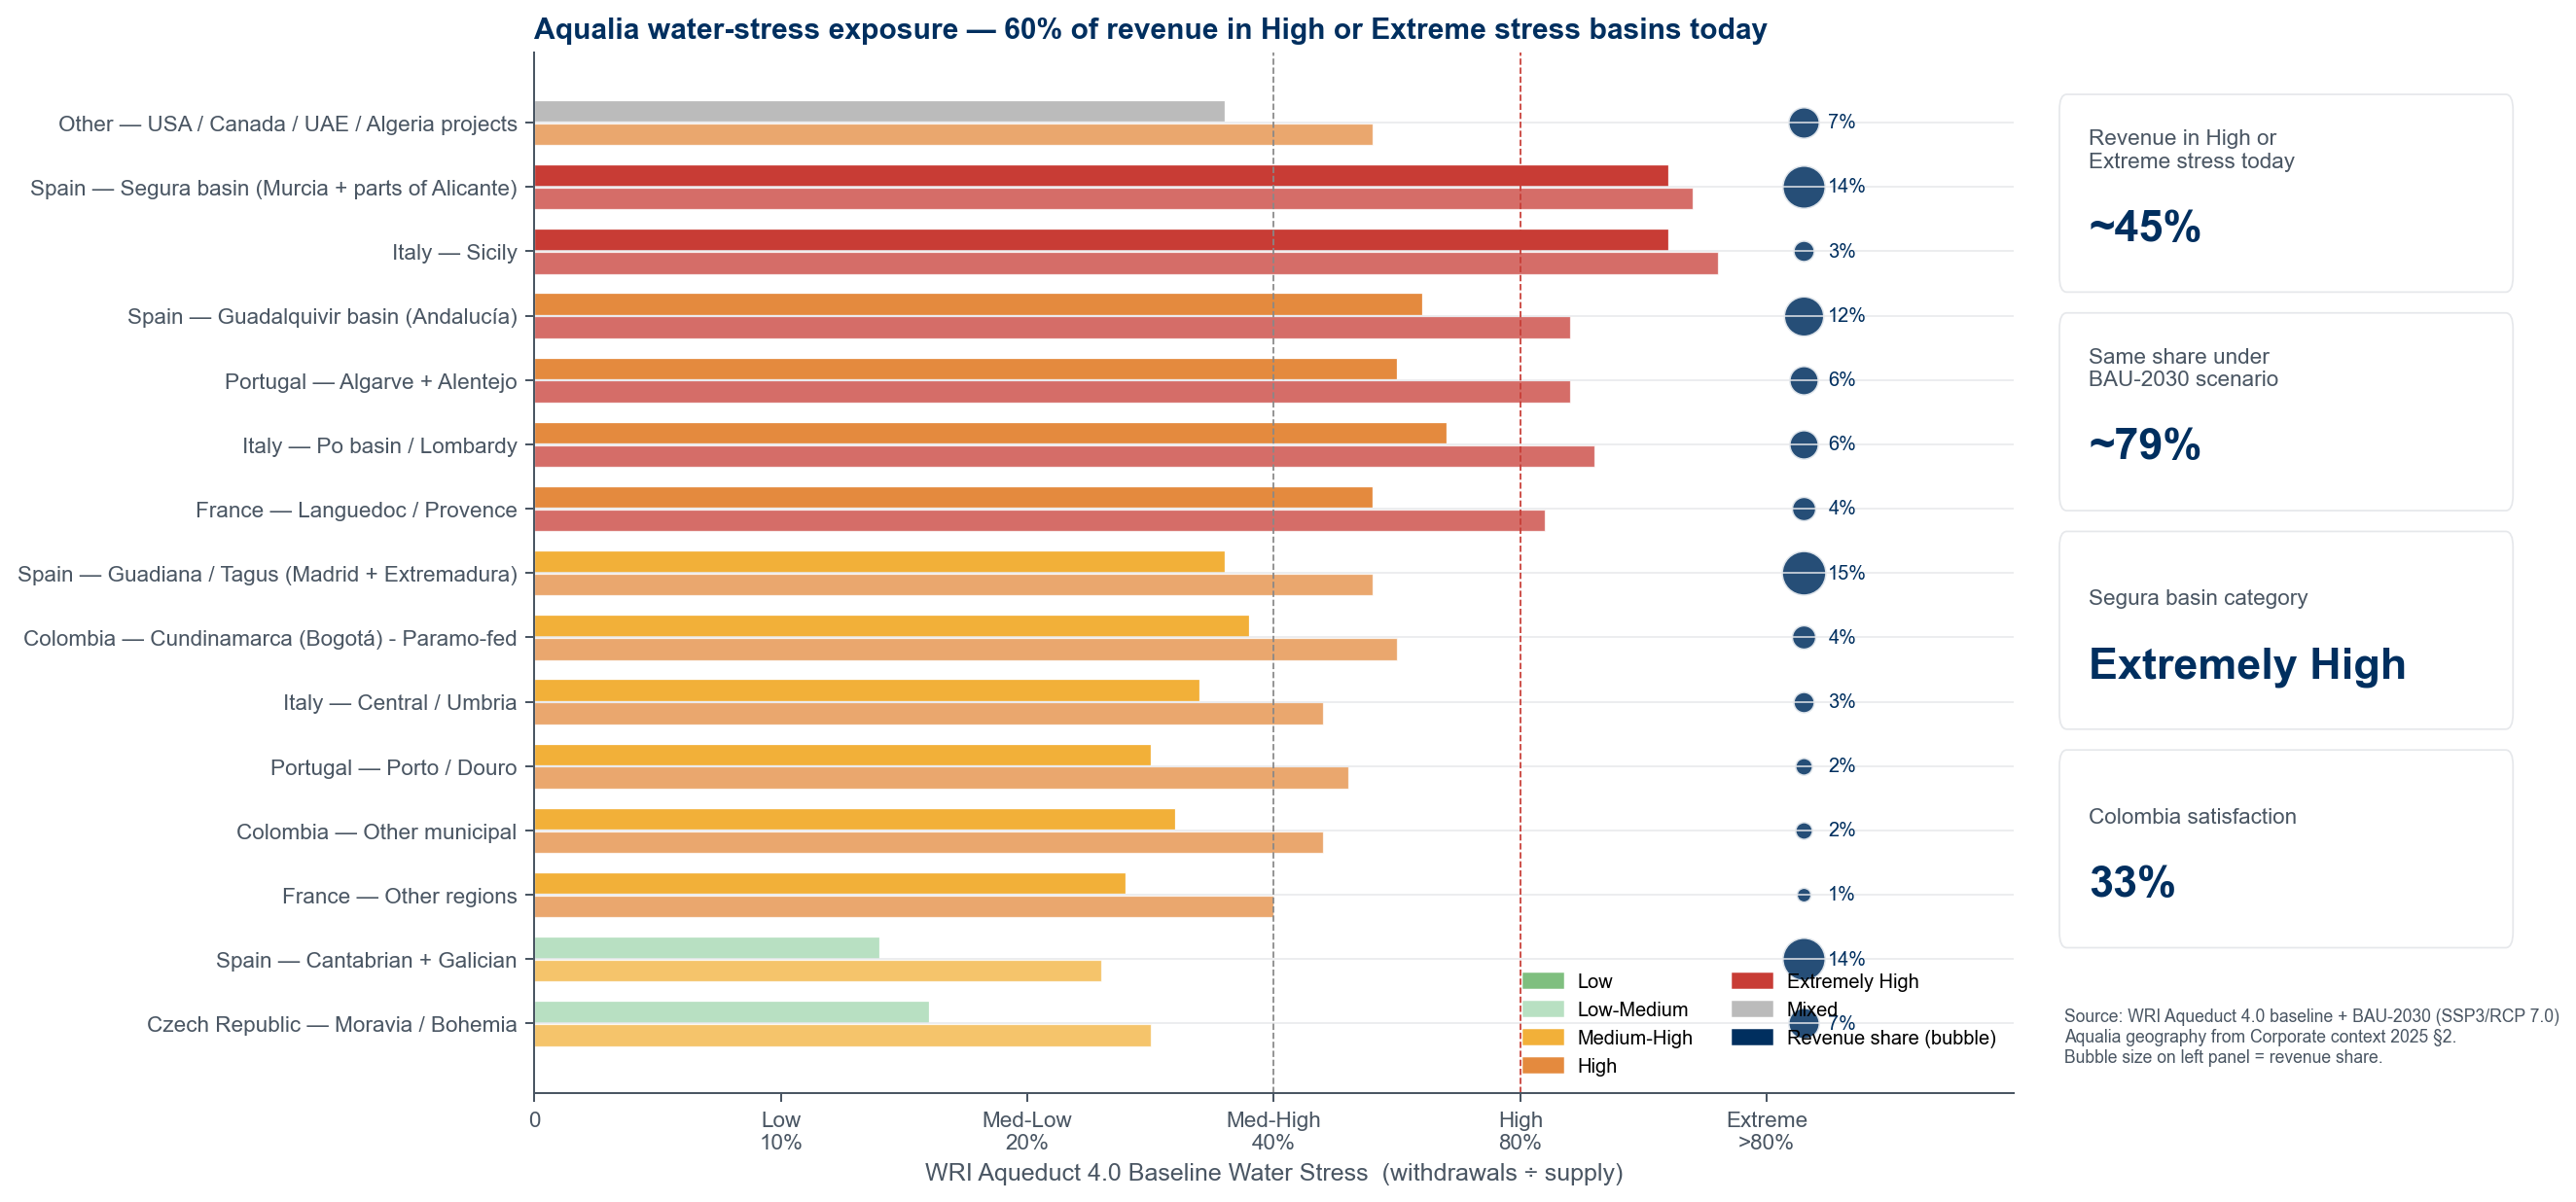
\includegraphics[width=0.9\textwidth]{aqueduct_exposure.png}
\caption[WRI Aqueduct water-stress exposure]{Baseline water stress by Aqualia concession basin, WRI Aqueduct~4.0, 2024 baseline and BAU-2030. 45\% of revenue in High/Extreme stress today; 79\% in 2030.}
\label{fig:aqueduct}
\end{figure}

\subsection{The \euro{}500~M green bond programme}

The 2027--2030 CAPEX implied by Aqualia's Risk Map and our three topics totals \sig{\euro{}440~M} base case (\euro{}285--685~M under low/high assumptions). We recommend funding via a \sig{\euro{}500~million EU-Taxonomy-aligned green / sustainability-linked bond programme}, in four tranches aligned to CAPEX drawdown: \euro{}150~M (2027), \euro{}150~M (2028), \euro{}120~M (2029), \euro{}80~M (2030). At a 25~bp coupon spread~\cite{cbi2024}, the programme delivers \sig{\euro{}31~M of present-value interest savings} over a 10-year tenor (4.00\% vanilla vs 3.75\% green; 8\% discount rate; $500 \times 25\,\text{bp} \times A(10, 8\%) \approx$ \euro{}8.4~M nominal annual saving; PV $\approx$ \euro{}31.1~M). Conservative: the spread regularly exceeds 25~bp in Iberian and Italian issuance~\cite{icma2024}.

%% ========================================================================
\section{The Matrix and What It Tells Us}
\label{sec:matrix}

\subsection{Matrix structure}

The matrix plots Impact Severity (y-axis, inside-out) against Financial Severity (x-axis, outside-in), each on a 1--5 scale; the Target Zone is the top-right quadrant with both axes $\geq 2.5$. Each topic appears as a 90\% confidence ellipse from 10{,}000 Monte Carlo draws (Figure~\ref{fig:matrix}).

\begin{figure}[h]
\centering
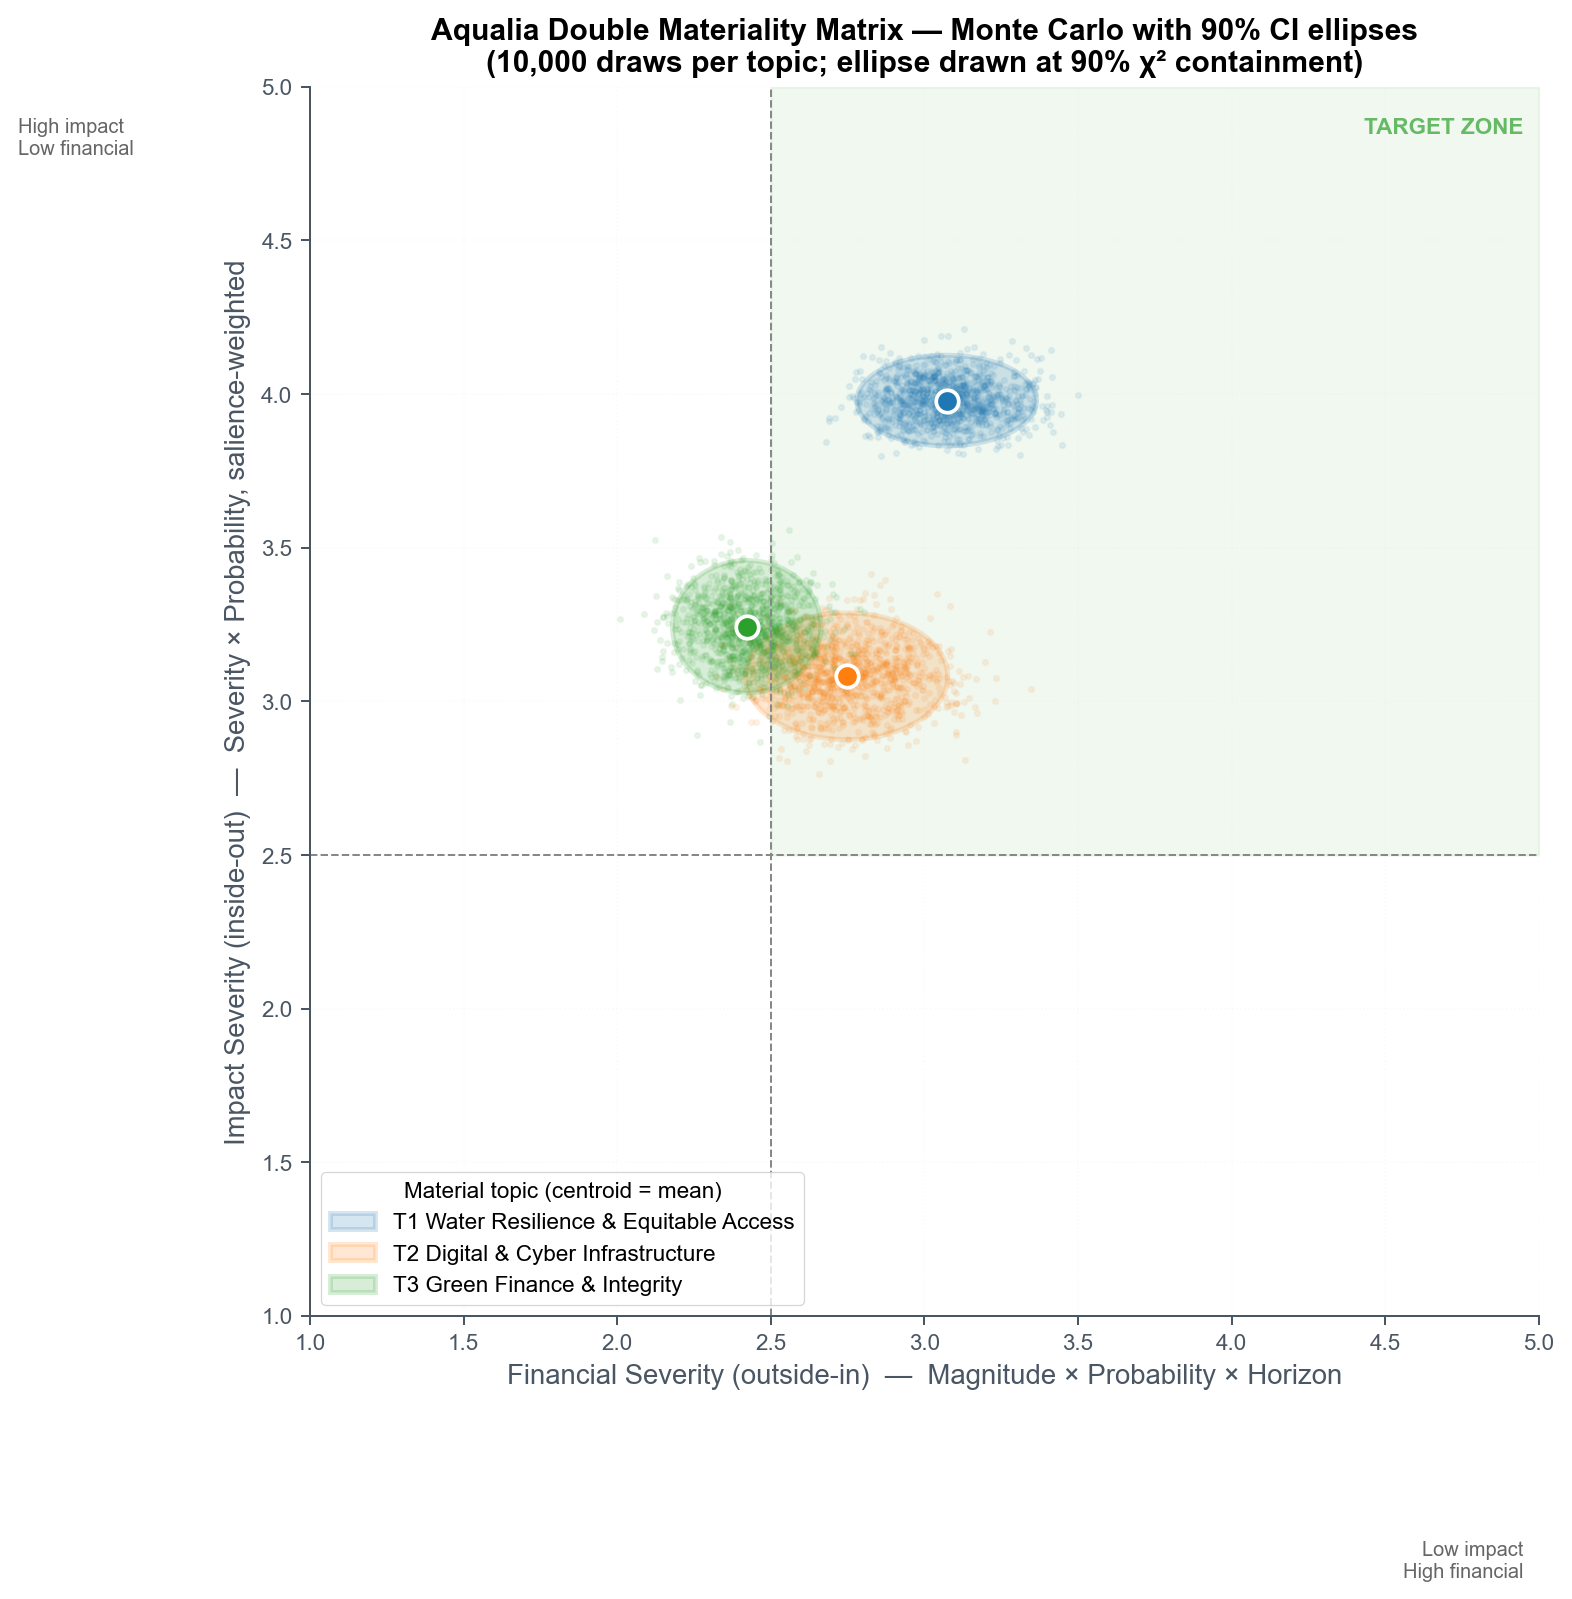
\includegraphics[width=0.82\textwidth]{matrix_mc.png}
\caption[Double materiality matrix]{Aqualia double materiality matrix. 90\% $\chi^2$ confidence ellipses from 10{,}000 Monte Carlo draws per topic. Target Zone shaded at both axes $\geq 2.5$. T1 solidly inside; T2 inside (our repositioning of the blind-spot cluster); T3 borderline on the financial axis, conditionally material.}
\label{fig:matrix}
\end{figure}

\paragraph{T1 (3.07, 3.98).}
Ellipse wholly inside Target Zone, bounded well away from both thresholds. Robust material under every test run.

\paragraph{T2 (2.75, 3.08).}
Ellipse inside Target Zone; financial-axis $p_5 = 2.50$, right on the boundary. Target Zone membership is directly attributable to our repositioning of the blind-spot cluster. Under Aqualia's original qualitative framework (2~IROs on Digitalisation), T2 would not be material; under our methodology it is.

\paragraph{T3 (2.42, 3.24).}
Centroid lies 0.08 below the financial threshold; $p_{95} = 2.61$, $p_5 = 2.24$. Conditionally material: Target Zone on impact, borderline on finance. This is the most informative methodological outcome, distinguishing robustly from conditionally material topics where a qualitative framework would paint both the same colour.

\subsection{Sensitivity drivers}
\label{ssec:sensitivity}

Top inputs by absolute swing per topic:
\begin{itemize}
\item \textbf{T1.} R-stress-revenue magnitude (financial); E1-adaptation probability (impact); O-reuse-market magnitude; R-CAPEX-UWWTD magnitude.
\item \textbf{T2.} Tech-pace probability (impact); O-tender-uplift magnitude (financial); R-digital-CAPEX magnitude.
\item \textbf{T3.} Compliance-CSDDD probability (impact); Green-finance-access probability; O-green-bond-premium magnitude.
\end{itemize}

\subsection{Robustness}

Under four alternate stakeholder-weighting schemes (Equal, Regulator-heavy, Community-first, Investor-first), no topic flips Target-Zone status: T1 remains in; T2 remains in; T3 remains borderline. Stability follows from top-$k$ aggregation: the most material subset drives position and is insensitive to modest re-weighting.

%% ========================================================================
\section{Strategic Sustainability Roadmap 2027--2030}
\label{sec:roadmap}

\subsection{Owned. Measurable. Aligned.}

Every recommendation is assigned to a named Executive Committee role from Aqualia's own Risk Map, pinned to a quantitative KPI, and anchored to an ESRS disclosure. The roadmap is structured as a 3-topic $\times$ 4-year grid (Table~\ref{tab:roadmap}).

\begin{table}[h]
\centering
\footnotesize
\caption{Strategic Sustainability Roadmap, 2027--2030. Each cell: action $\cdot$ KPI $\cdot$ named owner.}
\label{tab:roadmap}
\renewcommand{\arraystretch}{1.35}
\begin{tblr}{colspec={Q[l,t,wd=0.8cm] Q[l,t,wd=3.15cm] Q[l,t,wd=3.15cm] Q[l,t,wd=3.15cm] Q[l,t,wd=3.15cm]}, rowsep=1pt, colsep=4pt}
\toprule
 & \textbf{2027} & \textbf{2028} & \textbf{2029} & \textbf{2030} \\
\midrule
\rowcolor{white}
{\bfseries\color{tOne}T1} &
Restore S3 + Colombia review.\newline sat.\ $\geq 60\%$.\newline Director Spain/EU/Am.\ &
Segura basin reuse pilot.\newline NRW $-3$~pp.\newline Director Studies \& Ops. &
Italy adaptation CAPEX (Po).\newline tCO$_2$e/m$^3$ $-10\%$.\newline Director Spain/EU/Am.\ &
Reuse $\geq 25\%$ of WW; RD~1985/2024.\newline WFD clean.\newline Sustainability Dir. \\
{\bfseries\color{tTwo}T2} &
Digital twin Phase~1 (3 concessions).\newline coverage $\geq 80\%$.\newline CIO. &
OT/IT segmentation + NIS2 audit.\newline readiness $\geq 90\%$.\newline CIO. &
AI demand prediction rollout.\newline leak MTTR $-30\%$.\newline Dir.\ Strategy. &
Cyber MTTR $<$~4~h.\newline $\sim$~1\% revenue cyber spend.\newline CIO. \\
{\bfseries\color{tThree}T3} &
Tranche~1: \euro{}150~M.\newline Taxonomy alignment report.\newline CFO. &
Tranche~2: \euro{}150~M.\newline CSRD limited assurance.\newline CFO + Sust.\ Dir. &
Tranche~3: \euro{}120~M.\newline ISO~14001:2026 group-wide.\newline CFO. &
Tranche~4: \euro{}80~M.\newline TCFD + TNFD reasonable assurance.\newline CFO + Sust.\ Dir. \\
\bottomrule
\end{tblr}
\end{table}

\subsection{Integration with Aqualia's existing strategic plan}

Aqualia's 2024--2026 Strategic Sustainability Plan (PESA) operates along seven strategic lines (SL1 Climate Emergency through SL7 Partnerships). Our roadmap is designed to \emph{extend} PESA into 2027--2030 rather than replace it: T1 extends SL1 (Climate); T2 extends SL2 (Technology for Integrated Management); T3 extends SL4 (Financial \& Business Strategy) and SL5 (Ethics \& Compliance). The cross-walk between our twelve quarterly milestones and PESA's seven lines is fully traceable.

\subsection{Governance and reporting cadence}

We recommend Aqualia's Sustainability Committee adopt a \nav{semi-annual matrix refresh} using the reproducible Monte Carlo pipeline. Each refresh produces updated confidence ellipses; material shifts across two consecutive refreshes trigger Executive Committee review. This institutionalises the methodology rather than treating it as a one-off deliverable.

%% ========================================================================
\section{Limitations, Reverse Stress Test, and Ethical Framing}
\label{sec:limits}

\paragraph{Six limitations.}
\emph{(i)}~No external stakeholder consultation this cycle (mirrors Aqualia's own 2025 choice); the MAW salience model is a \emph{substitute}, not a \emph{replacement}. \emph{(ii)}~No asset-level financial disclosures; our \euro{}-ranges triangulate public segment data, peer benchmarks, regulatory cost factors. \emph{(iii)}~Real Options exhibit (desalination vs reuse) is illustrative; final numbers require Aqualia's asset-level WACC. \emph{(iv)}~ESRS heatmap uses TF--IDF, not dense embeddings; a one-line swap preserves findings while improving precision. \emph{(v)}~Aqueduct overlay uses public baseline data, not a commissioned hydrological model. \emph{(vi)}~Monte Carlo perturbation $\pm 0.7$ is a methodological judgement; sensitivity at $\pm 1.0$ is reported in the assumption log and rankings are stable.

\paragraph{Reverse stress test.}
\emph{T1} exits the Target Zone only under simultaneous downward revision of A03 (water-stress revenue $<40\%$), A04 (reuse market $<$~\euro{}15~M), and E1-adaptation probability to~2 --- a conjunction implausible given WEF~\cite{wef2025} and EU policy consensus. \emph{T2} exits only if O-tender-uplift magnitude drops to~1 \textbf{and} R-cyber-incident probability drops to~1 --- both contradicted by empirical data. \emph{T3} is the sensitive topic: conditions that \emph{push T3 into} the Target Zone include Omnibus-I rollback milder than expected, CoC spread widening beyond 25~bp, and Aqualia issuance timing concentrated in higher-spread windows.

\paragraph{Ethical framing.}
We attribute all IRO counts, scoring formulas, and the sixteen material topics to Aqualia's 2025 Double Materiality Review~\cite{aqualiaDMReview2025, aqualiaMethodology2025}. Our contribution is a methodological extension, not a replacement. All benchmark material is publicly disclosed. Where we identify gaps, the framing is corrective rather than adversarial; the purpose is to strengthen Aqualia's framework, which is already among the most mature in the Spanish water sector.

%% ========================================================================
\section{Conclusion}
\label{sec:conclusion}

Three material topics. \euro{}18~million per year of recurring financial materiality un-priced by the current framework. A \euro{}500~million EU-Taxonomy-aligned green bond programme, four tranches 2027--2030, that funds the implied \euro{}440~million CAPEX and captures \euro{}31~million of present-value interest savings. Every milestone owned. Every KPI quantified. Every disclosure ESRS-anchored.

Aqualia has delivered clean water across Europe and Latin America since 1894. Climate is rewriting the economics of water under them. In 2030, when a tap opens in Cartagena, or Rome, or Murcia, or Prague, it should open with confidence: not because the water happened to arrive, but because someone planned for the climate that came. That is what we mean by \emph{water as strategy, not water as reporting}.

%% ========================================================================
\clearpage
\appendix

\section*{Appendices}
\addcontentsline{toc}{section}{Appendices}
\renewcommand{\thesection}{\Alph{section}}
\setcounter{section}{0}

\section{Scoring Thresholds (summary)}
\label{app:thresholds}

Full version at \texttt{03\_analysis/scoring\_rubric.md}. Each sub-criterion (Scale, Scope, Remediability, Probability, Magnitude) documented with 1--5 thresholds, water-sector calibrations, and cited sources.

\begin{center}
\footnotesize
\renewcommand{\arraystretch}{1.2}
\begin{tblr}{colspec={Q[l,t,wd=1.9cm] Q[l,t,wd=1.2cm] Q[l,t,wd=3.2cm] Q[l,t,wd=3.1cm] Q[l,t,wd=2.6cm] Q[l,t,wd=1.6cm]}, rowsep=1pt, colsep=4pt}
\toprule
\textbf{Criterion} & \textbf{Band 1} & \textbf{Band 3 (Moderate)} & \textbf{Band 5 (Severe)} & \textbf{Anchor} & \textbf{Source} \\
\midrule
Scale       & Marginal  & Noticeable, reversible         & Systemic, catastrophic             & ESRS~1~\S 43--47 & \cite{esrs2023} \\
Scope       & Single site & Multiple sites / region      & Group-wide / multi-country         & EFRAG~IG-1       & \cite{efrag2024} \\
Remediability & $<$~1~year & 1--5~years, partial         & $>$~10~years / irreversible        & EFRAG~IG-1~\S 69 & \cite{efrag2024} \\
Probability & Remote     & Possible                       & Near-certain                       & MAW~(1997)        & \cite{mitchell1997} \\
Magnitude   & $<$~0.1\% rev & 0.5--2\% rev (\euro{}7--28~M) & $>$~5\% rev (\euro{}70~M+)         & Aqualia rev.\ A01 & \cite{aqualiaSR2024} \\
\bottomrule
\end{tblr}
\end{center}

\section{Assumption Log (A01--A17)}
\label{app:assumptions}

\begin{center}
\footnotesize
\renewcommand{\arraystretch}{1.2}
\begin{tblr}{colspec={Q[l,t,wd=0.6cm] Q[l,t,wd=9.4cm] Q[l,t,wd=5.0cm]}, rowsep=1pt, colsep=4pt}
\toprule
\textbf{Ref} & \textbf{Description} & \textbf{Primary source} \\
\midrule
A01 & Aqualia 2024 revenue anchor (conservative \euro{}1.4~B; disclosed \euro{}1{,}674.7~M) & Aqualia SR~2024 p.~103~\cite{aqualiaSR2024} \\
A02 & FCC Group segment share Aqualia $\approx 28\%$                                     & FCC URD 2024 \\
A03 & T1 revenue-at-water-stress-risk \euro{}25--110~M                                     & WRI Aqueduct~4.0~\cite{aqueduct2023} \\
A04 & T1 reuse-market upside \euro{}15--75~M                                              & RD~1985/2024~\cite{rd1985} \\
A05 & T1 OPEX under UWWTD recast \euro{}8--32~M/yr                                        & UWWTD recast~\cite{uwwtd2024} \\
A06 & T1 2027--2030 CAPEX \euro{}220--520~M                                              & Peer disclosures \\
A07 & T1 contingent liabilities \euro{}10--65~M                                           & WFD enforcement data \\
A08 & T2 cyber-incident revenue risk \euro{}12--80~M                                      & IBM Cost of a Data Breach 2024~\cite{ibm2024} \\
A09 & T2 digital-tender upside \euro{}8--45~M                                             & Peer URDs \\
A10 & T2 cyber \& digital OPEX \euro{}4--14~M/yr                                          & Gartner water-utility benchmark \\
A11 & T2 digital-twin CAPEX \euro{}45--130~M                                              & SWAN Forum benchmark \\
A12 & T2 GDPR/NIS2 contingent \euro{}5--56~M                                               & GDPR~\cite{esrs2023}; NIS2 \\
A13 & T3 ESG-laggard CoC spread \euro{}8--50~M                                            & MSCI 2024~\cite{msci2024} \\
A14 & T3 green-bond coupon saving \euro{}6--28~M                                          & CBI 2024~\cite{cbi2024} \\
A15 & T3 CoC saving over refinancing cycle \euro{}4--24~M/yr                              & CBI 2024~\cite{cbi2024} \\
A16 & T3 compliance CAPEX \euro{}8--35~M                                                   & Deloitte CSRD readiness \\
A17 & T3 CSDDD civil-liability contingent \euro{}3--35~M                                   & CSDDD~\cite{csddd2024} \\
\bottomrule
\end{tblr}
\end{center}

\section{Peer Material-Topic Cross-Walk (extract)}
\label{app:peers}

Full fourteen-column matrix at \texttt{01\_research/peer\_benchmark.md}. The extract below maps Aqualia's sixteen topics against five peers on whether each is a declared material topic.

\begin{center}
\footnotesize
\renewcommand{\arraystretch}{1.15}
\begin{tblr}{colspec={Q[l,t,wd=4.3cm] Q[c,m] Q[c,m] Q[c,m] Q[c,m] Q[c,m] Q[c,m]}, rowsep=1pt, colsep=4pt}
\toprule
\textbf{Topic} & \textbf{Aqualia} & \textbf{Veolia} & \textbf{Suez} & \textbf{Saur} & \textbf{Facsa} & \textbf{G.~Omnium} \\
\midrule
Climate adaptation (E1)       & \cmark & \cmark & \cmark & \cmark & \cmark & \cmark \\
Water resource sustain.\ (E3) & \cmark & \cmark & \cmark & \cmark & \cmark & \cmark \\
Consumer \& service (S4)      & \cmark & \cmark & \cmark & \cmark & \cmark & \cmark \\
Own workforce (S1)            & \cmark & \cmark & \cmark & \cmark & \cmark & \cmark \\
Business conduct (G1)         & \cmark & \cmark & \cmark & \cmark & \cmark & \cmark \\
Affected communities (S3)     & \xmark & \cmark & \cmark & \cmark & \xmark & \cmark \\
Digitalisation (AQ)           & partial & \cmark & \cmark & \cmark & \cmark & \cmark \\
Cybersecurity (AQ)            & \cmark & \cmark & \cmark & \cmark & \xmark & \cmark \\
Green finance (AQ)            & \cmark & \cmark & \cmark & \xmark & \xmark & partial \\
Circular economy (E5)         & partial & \cmark & \cmark & \cmark & \cmark & \cmark \\
Biodiversity (E4)             & \cmark & \cmark & \cmark & \cmark & \cmark & \cmark \\
TNFD commitment               & \cmark & \cmark & \cmark & \xmark & \xmark & \xmark \\
\bottomrule
\end{tblr}
\end{center}

\section{Stakeholder Salience Scoring (Mitchell--Agle--Wood)}
\label{app:salience}

\begin{center}
\footnotesize
\renewcommand{\arraystretch}{1.2}
\begin{tblr}{colspec={Q[l,t,wd=4.8cm] Q[c,m] Q[c,m] Q[c,m] Q[l,m] Q[c,m]}, rowsep=1pt, colsep=4pt}
\toprule
\textbf{Stakeholder} & \textbf{P} & \textbf{L} & \textbf{U} & \textbf{Class} & \textbf{Weight} \\
\midrule
Public authorities \& regulators  & 1 & 1 & 1 & Definitive   & 0.120 \\
Customers \& end-users            & 1 & 1 & 1 & Definitive   & 0.120 \\
Shareholders (FCC / IFM)          & 1 & 1 & 1 & Definitive   & 0.120 \\
Employees (incl.\ unions)         & 1 & 1 & 1 & Definitive   & 0.120 \\
Investors \& analysts             & 1 & 1 & 0 & Dominant     & 0.080 \\
Suppliers \& subcontractors       & 1 & 1 & 0 & Dominant     & 0.080 \\
Business partners                 & 1 & 1 & 0 & Dominant     & 0.080 \\
Society / NGOs / media            & 0 & 1 & 1 & Dependent    & 0.080 \\
Local communities                 & 0 & 1 & 1 & Dependent    & 0.080 \\
Environment                       & 0 & 1 & 1 & Dependent    & 0.080 \\
Academia                          & 0 & 1 & 0 & Discretionary& 0.040 \\
\midrule
\textbf{Total}                    &   &   &   &              & \textbf{1.000} \\
\bottomrule
\end{tblr}
\end{center}

%% ========================================================================
\clearpage
\bibliography{references}

\end{document}
